\chapter{Architecture Design}
\label{chapter:intro}
This chapter gives an overview of the system design on the highest-level. Abstraction is used to cover the details which are not essential to outline what the system does and how the system works. \newline
The architecture outlines the structure, and interactions between a software and hardware subsystems. It is an essential element to understand the system. 

\section {Architecture Diagram}
The purpose of the architecture diagram is to provide a structural overview between the different system components. \\
\begin{figure}[h!]
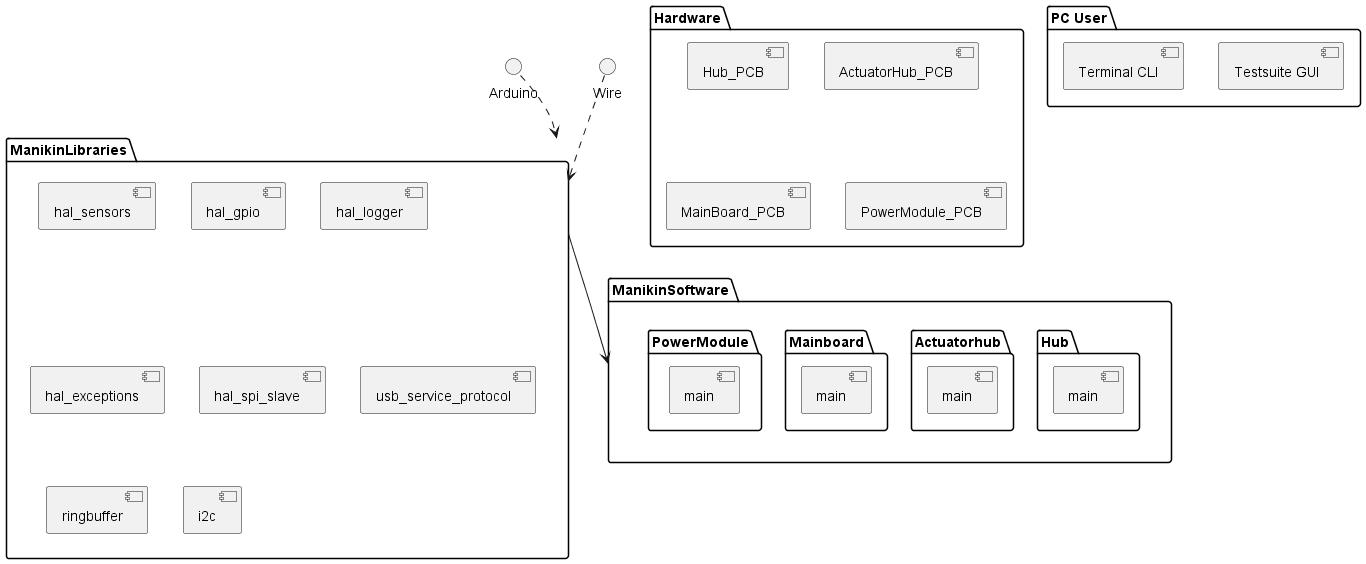
\includegraphics[scale=0.325]{figures/ArchitectureDiagram.png}
  \caption{Architecture diagram}
\end{figure}\\
The system architecture is broken down into four domain modules. Each domain is an independent entity and could function as it, this is the consequences (advantage) of the modular design.\\
The system architecture is organized into four distinct domain modules. Each module has an independent function and is an entity that is capable to operate autonomously. This modular approach enhances the flexibility, scalability and maintainability of the system. \\\\ 
By decoupling the hardware, software and user interface components, the system achieves an improvement in organization and maintainability. By minimizing dependencies between these parts, the impact of a error in one module reduces breaking other parts. This isolation of concerns makes integration process also smoother. 
\section {Data Flow}
The data flow within the Manikin system is illustrated in the figure below. The figure highlights the concise overview of how data is gathered, processed and logged. 
\begin{figure}[h!]
 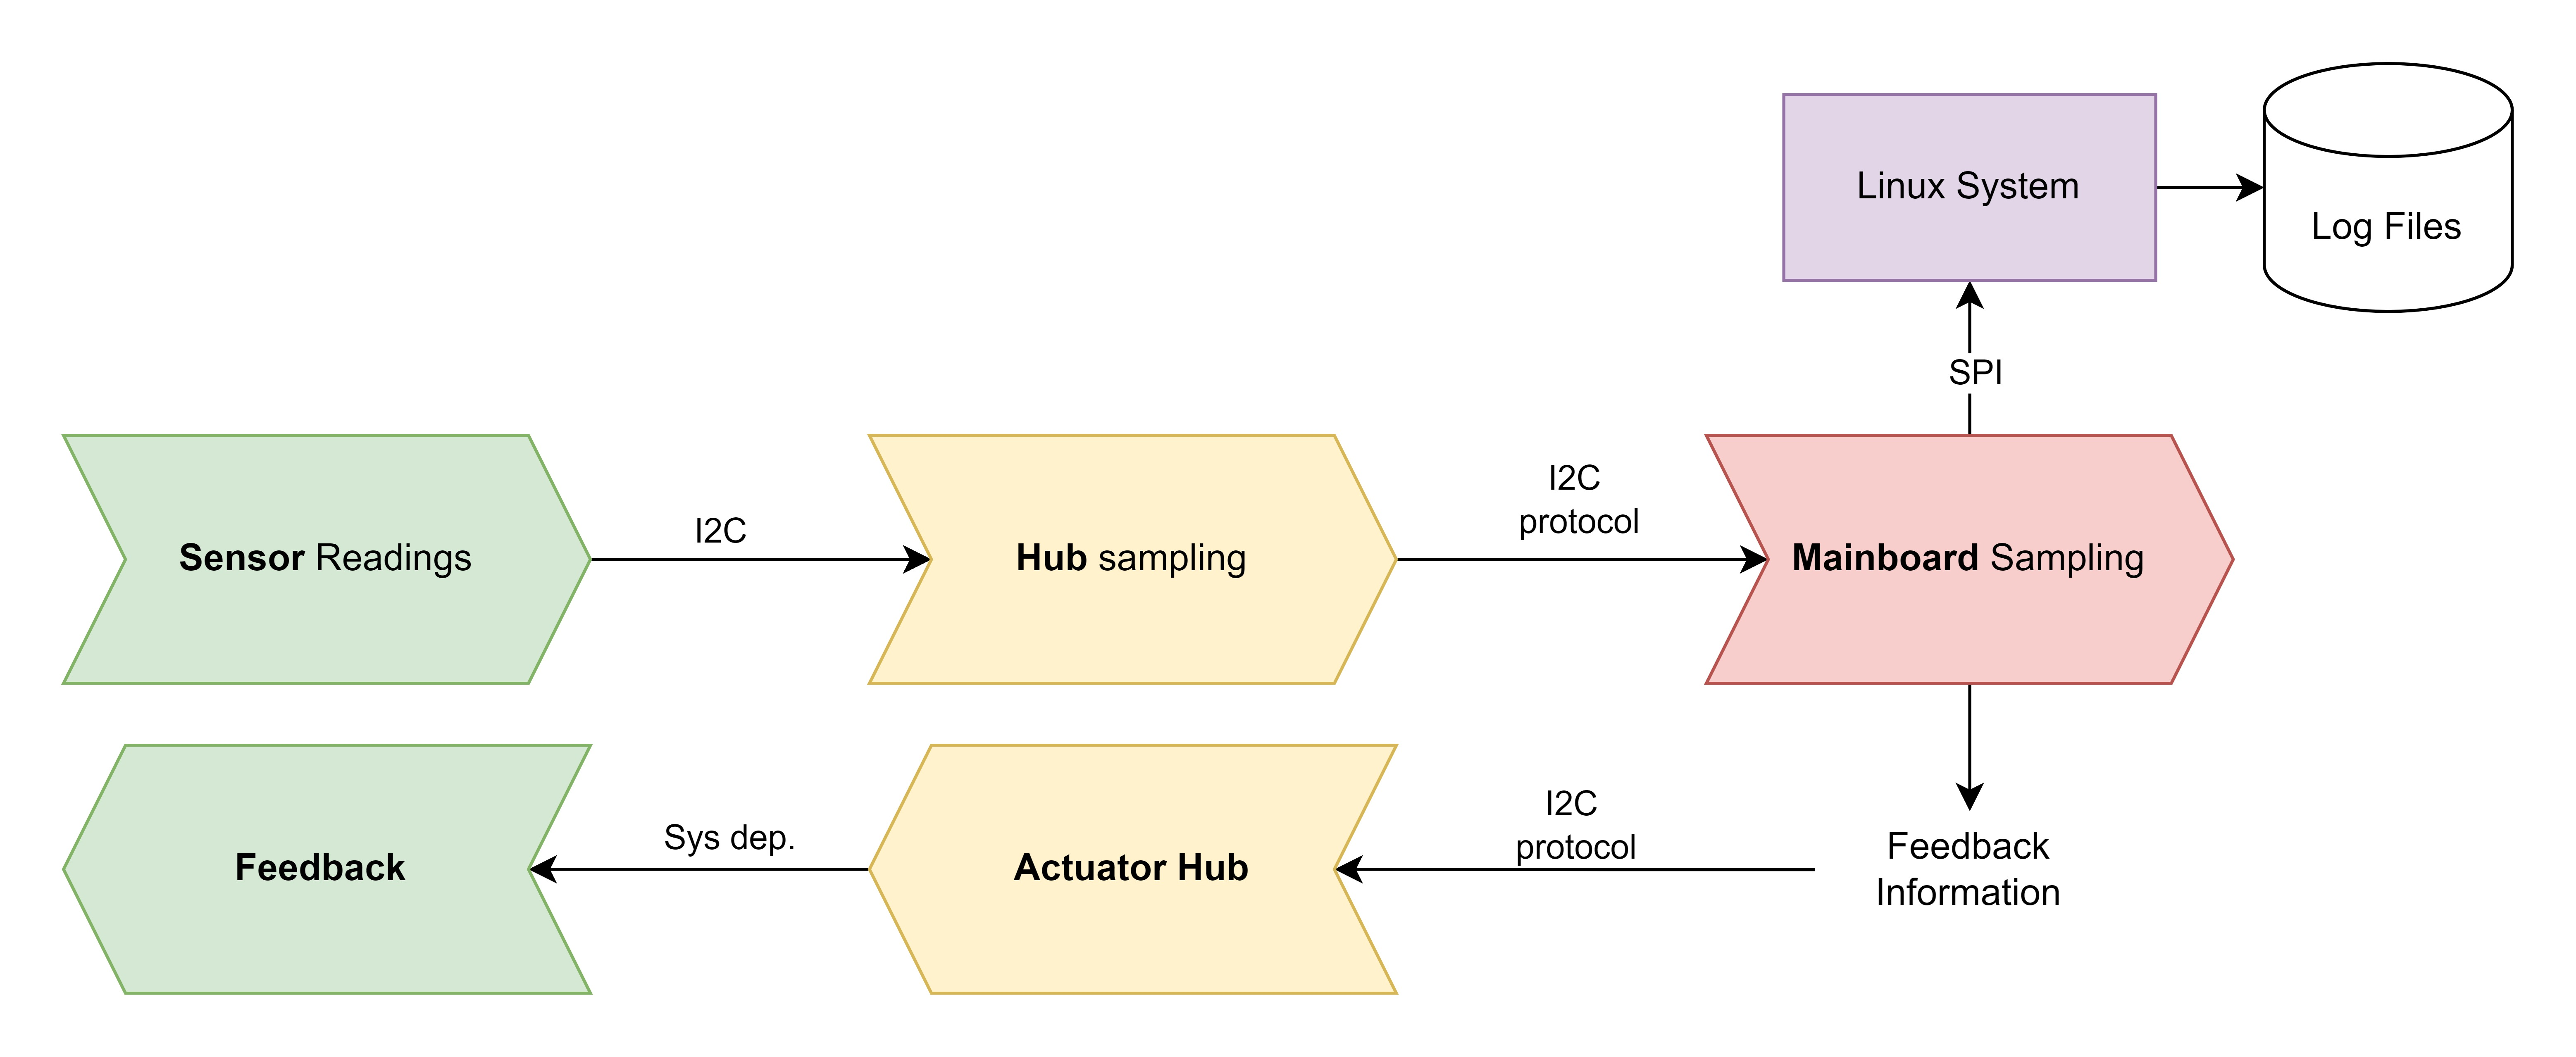
\includegraphics[scale=0.075]{figures/System Dataflow overview.jpg}
 \caption{Data flow diagram}
\end{figure}\\
The system begins by collection data from three sensors (currently), including compression, finger position and differential pressure sensors. These sensors capture relevant information about the user's training interaction and make them quantitative with physical measurements. The purpose of this is to create add valuable and quantitative performance insights, so that the feedback quality could be improved. \\\\
Next, the collected data is sampled and buffered by the hub, which serves as a intermediary component within the system. The hub is capable of buffering the data (sensor samples) locally. Besides local buffering the hub has also the ability to stream the data to a user device through a USB connection. This allows to make real-time monitoring and analysis of the gathered data. In this stage of the project, it will be used for validation of the data gathering.\\\\
Lastly, in the future the mainboard is going to save the data locally for the full training session. And also transmit the data to a single-board computer, which will handle the processing for an user interface solution. 
\\\\
One side note about the figure is that the feedback loop, is outside the scope of this project group. Still it is relevant information, because the semester 6 ESE group is working on this part of the project during this the same project period.  
\section {System Dependencies}
It is important to be aware of the dependencies that this system has, because it has a impact on the design choices. 
The system is dependent on the following libraries and frameworks: \\
- Arduino framework \\
- \href{https://github.com/FrankBoesing/FastCRC}{FrankBoesing/FastCRC} \\
- \href{https://github.com/BriscoeTech/Arduino-FreeRTOS-SAMD21}{FreeRTOS SAMD} \\
- Our own libraries - \href{https://github.com/RobotPatient/Manikin_Software_Libraries}{Manikin Software Libraries} \\
- \href{https://github.com/google/googletest}{GoogleTest and GMock} for unit testing \\
- Provided PCB and hardware.
\begin{table}[hb!]
\begin{tabular}{llll}
\cline{1-2} \cline{4-4}
\rowcolor[HTML]{000000} 
{\color[HTML]{FFFFFF} \begin{tabular}[c]{@{}l@{}}Depen-\\ dency \\ ID\end{tabular}} &
  {\color[HTML]{FFFFFF} \begin{tabular}[c]{@{}l@{}}Dependency\\ Naming\end{tabular}} &
  {\color[HTML]{FFFFFF} \begin{tabular}[c]{@{}l@{}}Establishment\\ Description\end{tabular}} &
  {\color[HTML]{FFFFFF} \begin{tabular}[c]{@{}l@{}}Implementation \\ Consequences\end{tabular}} \\ \hline
\multicolumn{1}{|l|}{DEP1} &
  \multicolumn{1}{l|}{\begin{tabular}[c]{@{}l@{}}Arduino \\ ecosystem\end{tabular}} &
  \multicolumn{1}{l|}{Clients want.} &
  \multicolumn{1}{l|}{\begin{tabular}[c]{@{}l@{}}- Performance is not optimized. \\ + Ability to rapid prototype due to\\ Arduino abstraction.\end{tabular}} \\ \hline
\multicolumn{1}{|l|}{DEP2} &
  \multicolumn{1}{l|}{Wire.h} &
  \multicolumn{1}{l|}{\begin{tabular}[c]{@{}l@{}}Fast prototyping \\ \& development need.\end{tabular}} &
  \multicolumn{1}{l|}{\begin{tabular}[c]{@{}l@{}}- Limited to small set of low-level I2C \\ implementation.\\ + Fast prototyping.\\ + Familiar communication implementation \\ for Arduino hobbyists.\end{tabular}} \\ \hline
\multicolumn{1}{|l|}{DEP3} &
  \multicolumn{1}{l|}{PlatformIO} &
  \multicolumn{1}{l|}{\begin{tabular}[c]{@{}l@{}}Arduino ecosystem \\ extra configuration\\ need.\end{tabular}} &
  \multicolumn{1}{l|}{\begin{tabular}[c]{@{}l@{}}- (new/next) developers need the know-how to \\ get started.\\ + Control of compilation and libraries version \\ imports etc.\\ + Decoupling from Arduino IDE! Ability to \\ use other IDE for example VScode.\end{tabular}} \\ \hline
\multicolumn{1}{|l|}{DEP4} &
  \multicolumn{1}{l|}{\begin{tabular}[c]{@{}l@{}}CMake\\\end{tabular}} &
  \multicolumn{1}{l|}{\begin{tabular}[c]{@{}l@{}}Needed for compling\\ and running of (mock) unit tests \\ without the DUT.\\ \end{tabular}} &
  \multicolumn{1}{l|}{\begin{tabular}[c]{@{}l@{}}- (new/next) developers need the know-how \\ and experience to get started. \\ + Configuration flexibility.\\ + Code building on dev device as well as for \\ target device.\\ + Easy test running option without changes\\  files or project. \\ \end{tabular}} \\ \hline
\end{tabular}
\caption{Dependency list overview}
\label{tab:dependency-list}
\end{table}\\

\section {System Connectivity Interfaces}
This section gives an general overview of all the system communication interfaces. \\ The technical implementation is documented in the next chapter.  

\subsection{USB Service}
The USB service feature serves the primary purpose of establishing a USB interface between the hub and a user device (PC). The main functionality is to enable data logging, allowing the system to transfer(stream) the gather data to the PC for storage, real-time analysis or further processing. This USB service provides a reliable and a compatible feature of communication and integration with PC-based applications and systems.

\subsection{Hub I2C}
The I2C interface plays a crucial role in the communication within the Manikin system. It has two distinct communication functionalities. \\\\
The first I2C feature enables communication between the sensors and the hub. This allows the hub to receive data from the various sensors, such as compression, finger position and differential pressure sensors. The I2C interface ensures reliable and efficient transmission of sensor data, enabling accurate measurements and feedback within the system. Sampling sensor data is a critical aspect of the system, so this part of the firmware is through-fully tested. \\\\ 
Secondly, the I2C interface facilitates data processing between the hub and the mainboard. Via this connection the hub can transfer buffered data and the system information to the mainboard. Vice versa, the mainboard could control the data gathering of the hub, think of configuring sampling rate or the sensor type on connected to a port. \\\\
In short, the I2C interface within the Manikin system serves as a vital communication technology, supporting data acquisition and processing between the hub and the mainboard.

\subsection{SPI Slave SBC}
The SPI slave protocol plays a role in enabling communication between the mainboard and the single-board computer. In the future the single-board computer will take care of data processing, logging and handling feedback logic. \\
The design of the SPI slave protocol takes this into consideration the future scalability and modularity requirements, ensuring its flexibility and robustness for upcoming advancements and potential expansions.
\pagebreak
\begin{figure}
    \section{Class Abstraction}
    \centering
    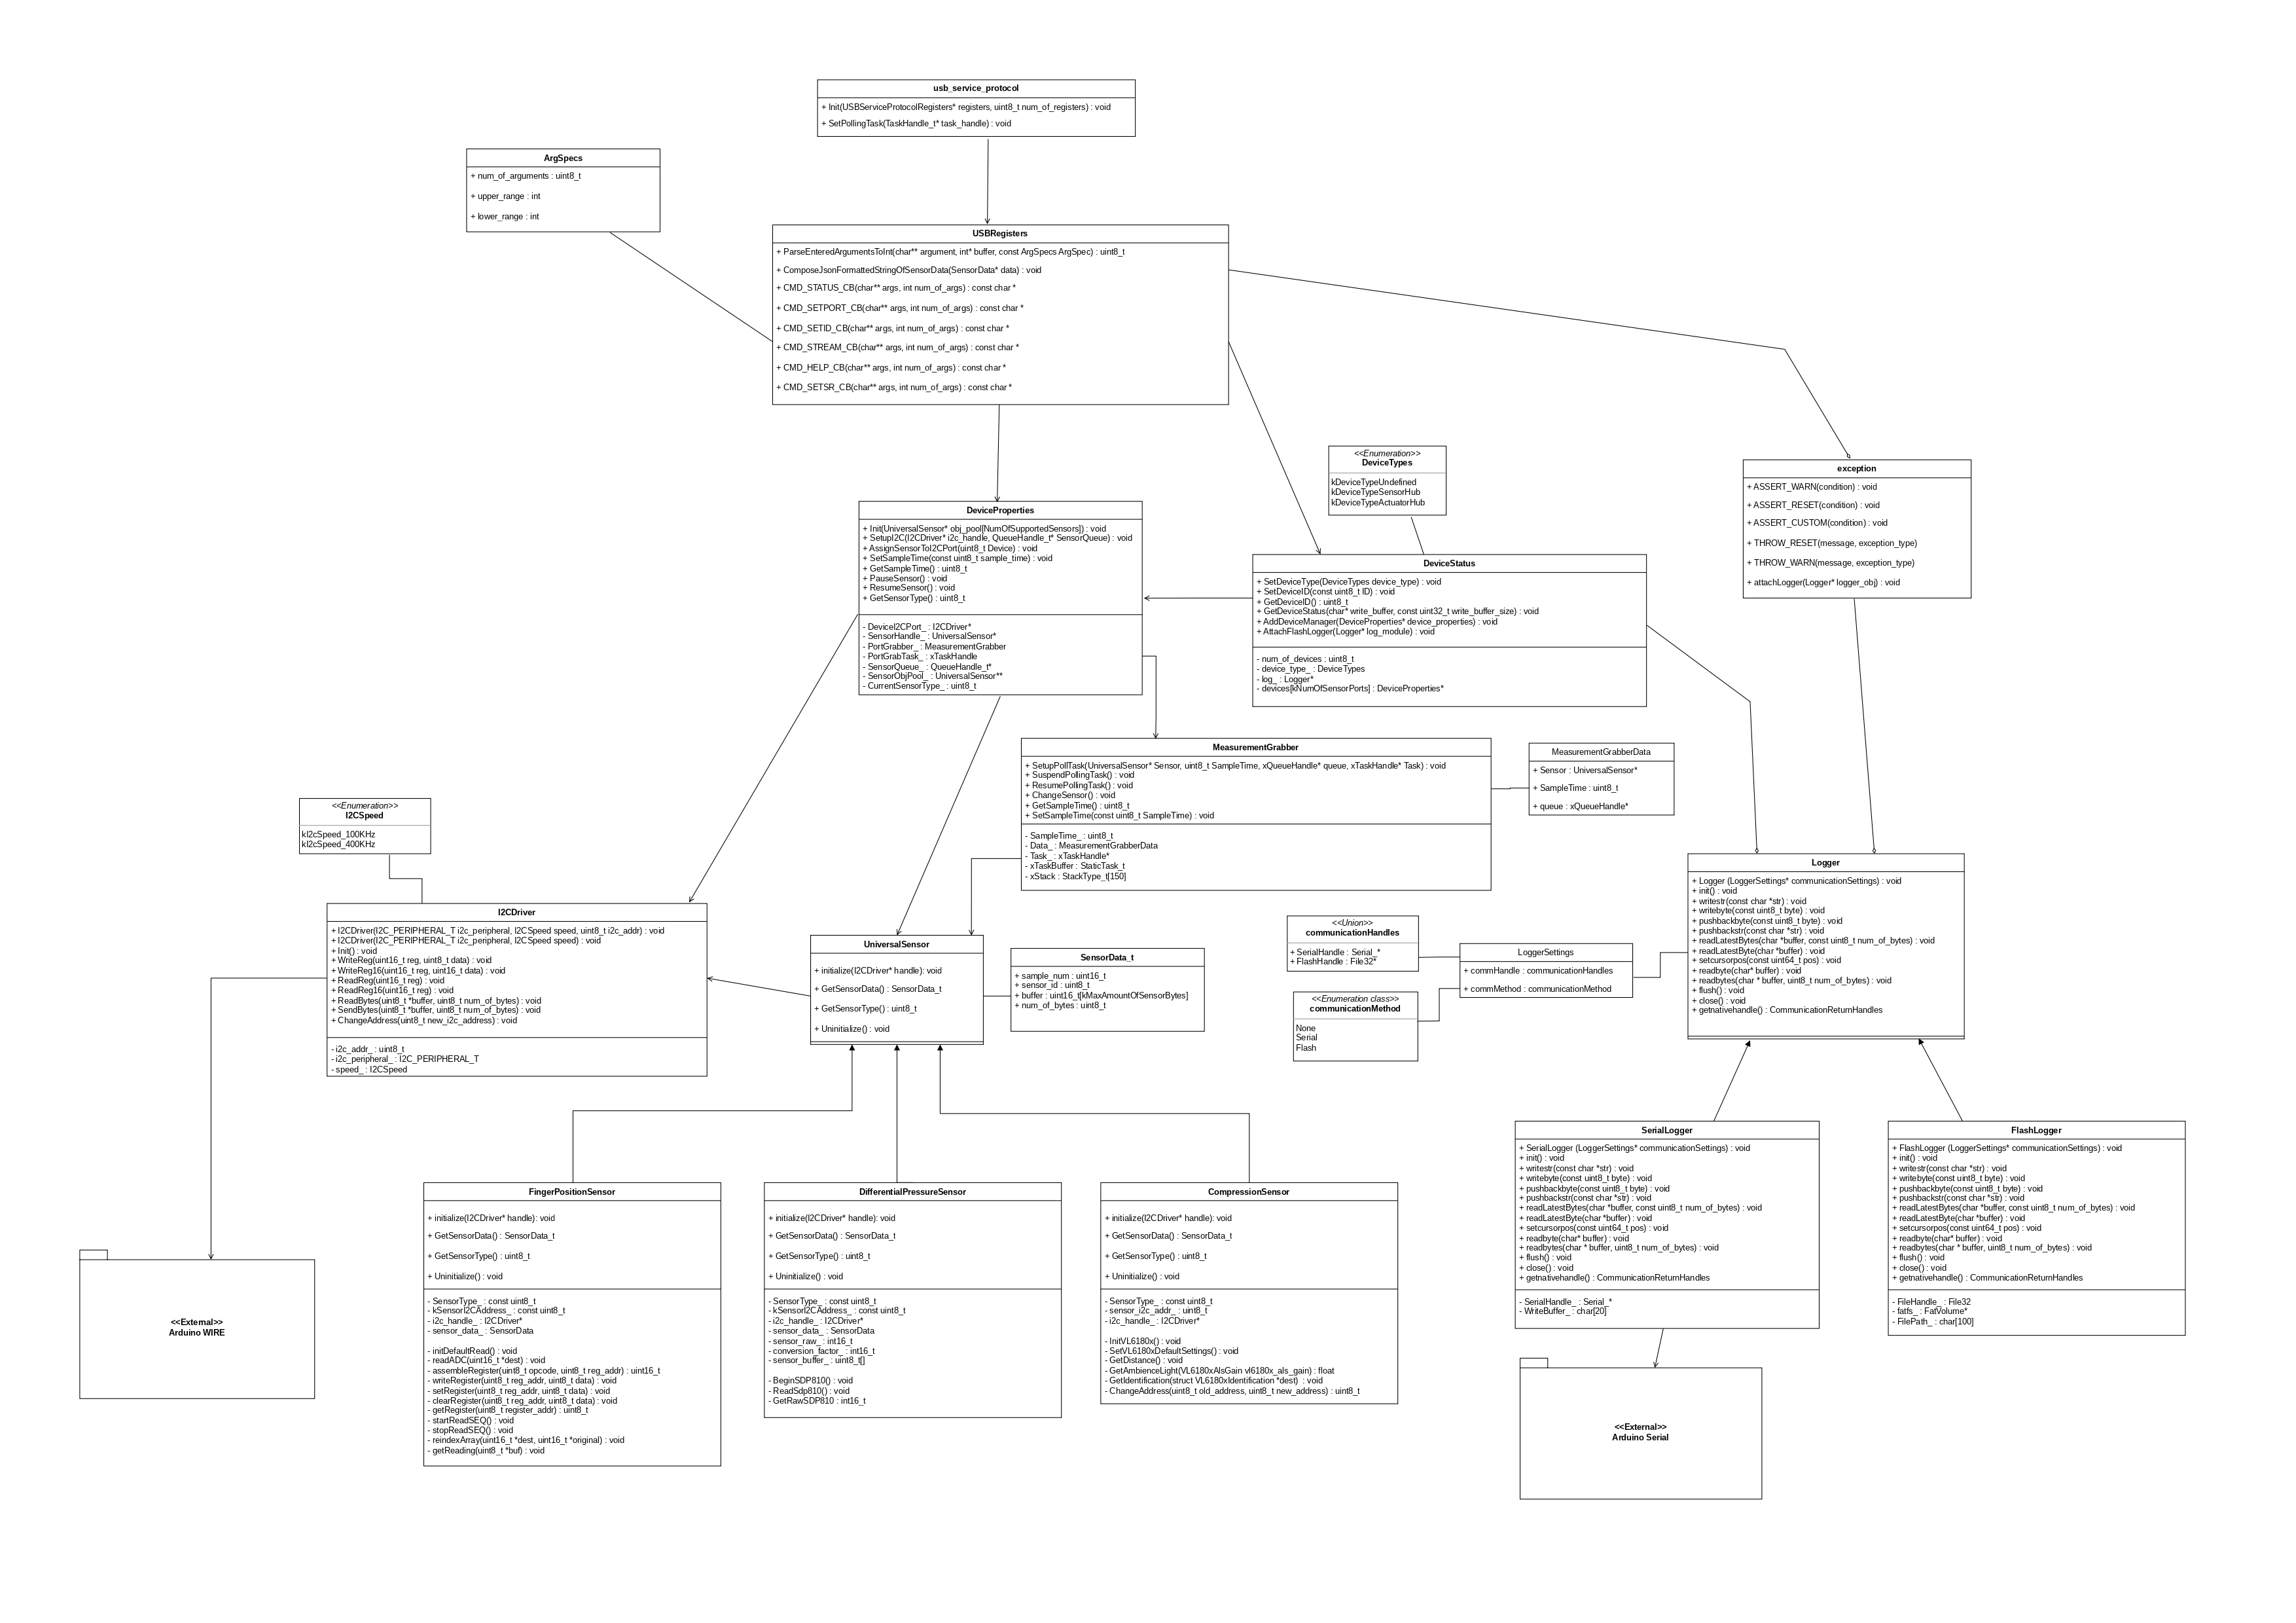
\includegraphics[scale=0.65]{figures/SensorHub_Class_Diagram.jpg}
    \caption{Class diagram of the SensorHub firmware}
    \label{fig:SensorHubClassDiagram}
\end{figure}
\section{Hierarchical Overview}
\begin{figure}[h!]
  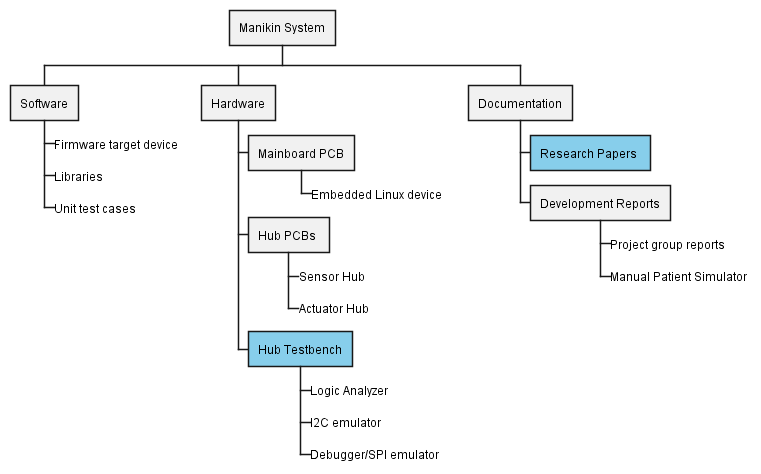
\includegraphics[scale=0.60]{figures/Hierarchial_Diagram.png}
  \caption{Hierarchical diagram}
\end{figure}
The Manikin project is composed of three main hierarchical levels: Software, Hardware, and Documentation development.\\
At the software level, there are three key components. The firmware target device which contains the software developed to the dedicated hardware device. General project libraries, which contains modular software modules that could be reused accross the devices.\\\\
The hardware level consists of PCB and electrical related development. The mainboard PCB serves as the central circuit board, and which contains a microcontroller and also a single-board computer. The hub PCBs are connected to the mainboard and aggregate data or are used for controlling a transducer to generate feedback. \\\\
Lastly, the documentation level encompasses resources vital for knowledge sharing and development. Also the main activity of the client, research, is included here because this activity has a impact on the system development. Insights from the research papers provide new needs, opportunities and ideas to develop new features and/or functionalities. \\ 
Development reports, include the contributions of temporary development teams for reference, system specification and information for the next development groups or phases.\\\\
In summary the hierarchical diagram illustrates the abstraction levels of the Manikin System. And gives an overview of the areas of research and development in the overall project.\\\\
Light blue boxes are outside of the project scope. The Hub Testbench is started in this project, but due to prioritization is set on hold. 
